\documentclass[12pt]{article}
\usepackage{graphicx}
\title{ElectroStatics 2}
\author{Britteny,Kishaun,Abhi}

\begin{document}
\begin{titlepage}
\begin{center}
	\textsc{\LARGE Rutgers University}\\[1.5 cm]
    \textsc{\Large Physics 2 lab}\\[0.5cm]
    \rule{\linewidth}{0.5mm} \\ [.4 cm]
    {\huge \bfseries ElectroStatics 2}\\[.4 cm]
    \rule{\linewidth}{0.5mm} \\ [1.5 cm]
    \begin{minipage}{0.4\textwidth}
	\begin{flushleft} \large
	\emph{Authors:}\\
	Brittney,Kishan,Abhi
	\end{flushleft}
	\end{minipage}
	\begin{minipage}{0.4\textwidth}
	\begin{flushright} \large
	\emph{Teacher:} \\
	James
	\end{flushright}
	\end{minipage}\\[2 cm]
	\textsc{ \Large Signatures} \\[1.7 cm] 
	\rule{10 cm}{0.5mm} \\ [2.0 cm]
	\rule{10 cm}{0.5mm} \\ [2.0 cm]
	\rule{10 cm}{0.5mm}
	\vfill
	{\large {July 19, 2013}}
\end{center}
\end{titlepage}

\section*{Part 1 - Amount of Charge}

\subsection*{procedure and goal}
	
	 We applied varying voltage sources to a spherical capacitor. We then measured the charge on the spherical capacitor.Our goal was to find the relationship between the voltage applied and charge measured. 
	 \begin{figure}[h]
	 \centering
	 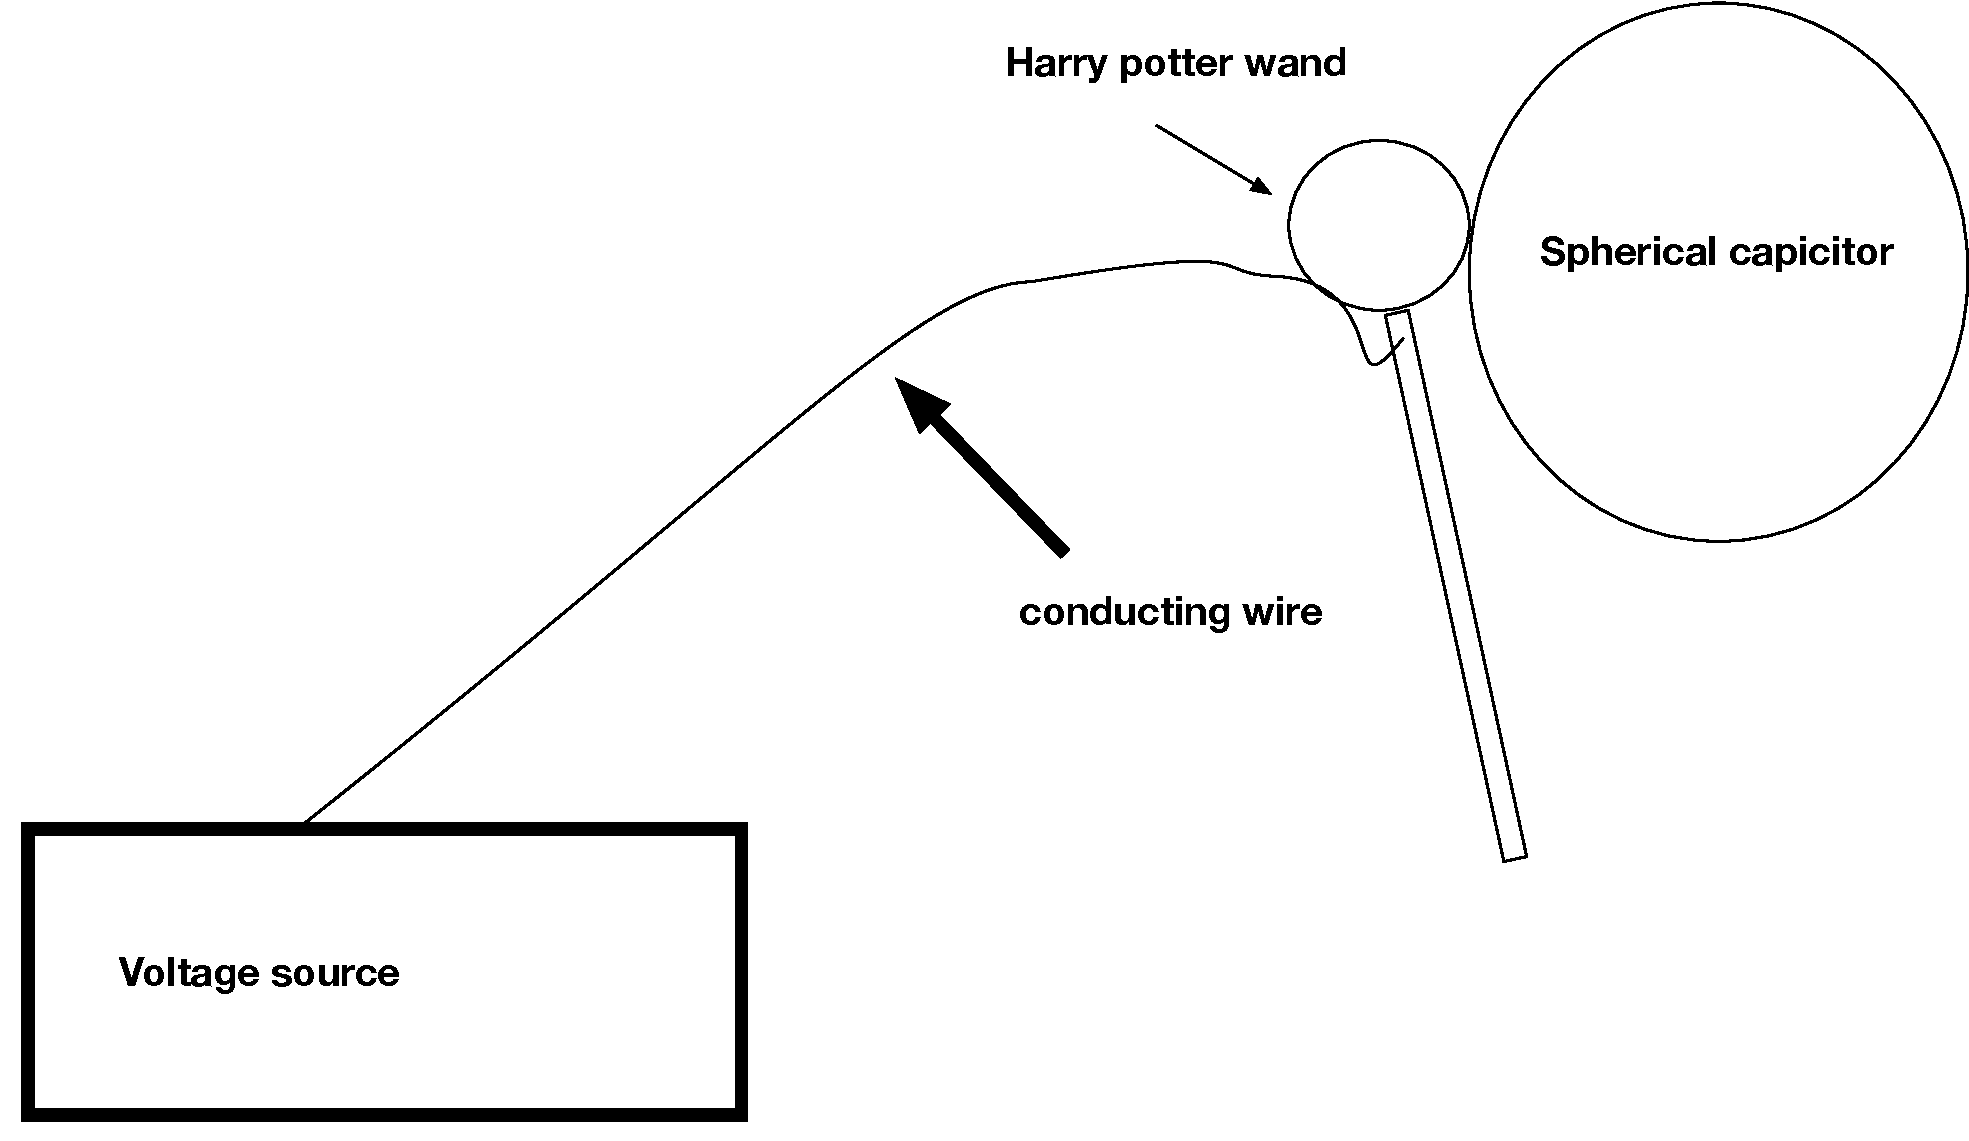
\includegraphics[scale = .4]{diagram1}
	 \caption{the setup to get current to the sphere}
	 \end{figure}


	 The harry potter wand is just there to transfer current to the sphere. It is not necessary but it is safer for students ;We could have connected the voltage source straight to the sphere. 

\subsection*{Prediction}
	From our knowledge of physics we know that charge travels from high potential to low potential. The \emph{voltage source} always has a fixed potential, while the Sphere has zero potential. But after the connection from the voltage source to the sphere is made, charge travels from the voltage source to the sphere until the sphere's potential equals the voltage source's. Because we know the capacitance and final potential of the sphere, we can calculate the amount of charge on the sphere Using the the formula $C = \frac{Q}{V}$ 
	\begin{eqnarray}
	C & = & 4\pi\epsilon_0R = 4 \pi *8.85*10^-12 *.045 = 5*10^-12\\
	Q &= & V * C = \mathbf{750} * 5 * 10^-12 = 3.75 \ nC \\
	Q &= & V * C = \mathbf{1500} * 5 * 10^-12 = 7.5 \ nC \\
	Q &= & V * C = \mathbf{3000} * 5 * 10^-12 = 15 \ nC \\
	Q &= & V * C = \mathbf{6000} * 5 * 10^-12 = 30 \ nC 
	\end{eqnarray}
	making a table we get
	\begin{quote}
	\begin{tabular}{|r|r|}
	\hline 
	voltage(v) & charge(nC) \\
	\hline 
	750 & 3.75 \\
	1500 & 7.5 \\
	3000 & 15 \\
	6000 & 30 \\
	\hline
	\end{tabular}
	\end{quote}

\subsection*{Results}
	Here are our results. The charge values here are the peak charged observed:
	\begin{quote}
	\begin{tabular}{|r|r|r|}
	\hline 
	voltage(v) & charge-predicted(nC) & charge-observed(nC) \\
	\hline 
	750 & 3.75 & 1.9 \\ 
	1500 & 7.5 & 2.9\\
	3000 & 15 & 4.1 \\
	6000 & 30 & 5.8 \\
	\hline
	\end{tabular}
	\end{quote}
	

\end{document}